\chapter{Results}
\section{Virtual Prototyping of Cell Signals}
During the course 
\subsection{Numerical investigation of immunomagnetic label density and size on quantitative magnetoresistive sensing of single cells and cell aggregates}
Signal Similarity For Cells With Varying Bead Coverages

Cross-Correlation between single dipole with sum magentic moment and surface covered with randomly distributed magnetic particles

simulation of cell rolling velocity and forces

%\\nas.ads.mwn.de\tuze\t03\AG-Hayden Studenten\00_Students\Johann Brenner\02_software\01-MRCyte\Magnetic cytometry signal modeling
\subsection{Single Cell Signal}

\begin{figure}
	\centering
	\subfloat{
		\subfigimg[height=145pt]{a}{Ressources/Simulation/Big2um}	
	} \hfill
	\subfloat{
		\subfigimg[height=145pt]{b}{Ressources/Simulation/Small2um}	
	} \\
	\vspace{\baselineskip}
	\subfloat{
		\subfigimg[height=145pt]{c}{Ressources/Simulation/Big4um}
	}\hfill
	\subfloat{
		\subfigimg[height=145pt]{d}{Ressources/Simulation/Small4um}	
	}
\capption{Coverage Dependent Signal Correlation}{Mean from 3 differently distributed particles, SEM (\textbf{a}) d = \SI{4}{\micro\meter} (\textbf{b}) d = \SI{4}{\micro\meter} (\textbf{c}) d = \SI{8}{\micro\meter} (\textbf{d}) d = \SI{8}{\micro\meter}}
\label{fig:sim:coverage}
\end{figure}

\begin{figure}
		\centering
	\subfloat{
		\subfigimg[height=150pt]{a}{Ressources/Simulation/CorrelationDiff2um}	
	} \hfill
	\subfloat{
		\subfigimg[height=150pt]{b}{Ressources/Simulation/CorrelationDiff4um}	
	}
\capption{Difference of Cross-Correlation at Maximum Coverage}{Mean from 3 different particle distributions at maximum coverage(\textbf{a}) d = \SI{4}{\micro\meter} (\textbf{b}) d = \SI{8}{\micro\meter}}
\label{fig:sim:CorrDiff}
\end{figure}

\subsection{Cell Aggregates}

\begin{figure}
	\centering
	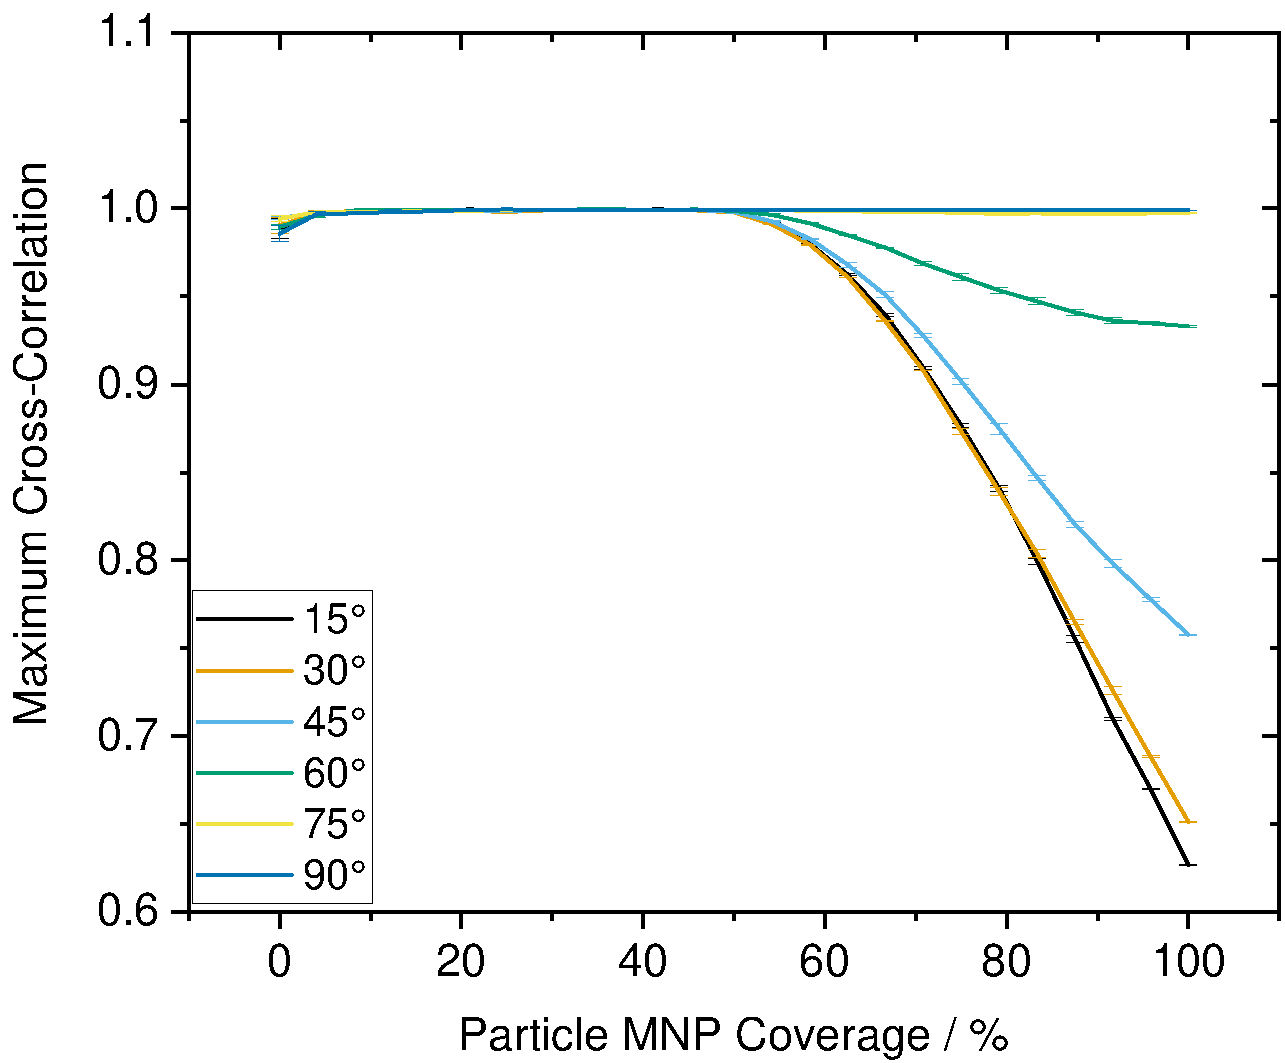
\includegraphics[width=.7\linewidth]{Ressources/Simulation/Aggregates}
	\capption{Sensor Signals Correlation between Two Cell Aggregates At Shifting Angles with a Reference Dipole}{Mean from 3 differently distributed particles, SEM}
\end{figure}

\section{Reference Bead Surface Functionalization}



\subsection{Amine-Surface Biotinylation}
Streptavidin-Atto488 reference calibration
Anti-Biotin-PE working?
BNF-Dextran-Streptavidin unspecific binding?



\begin{figure}[htb!]
	\centering
	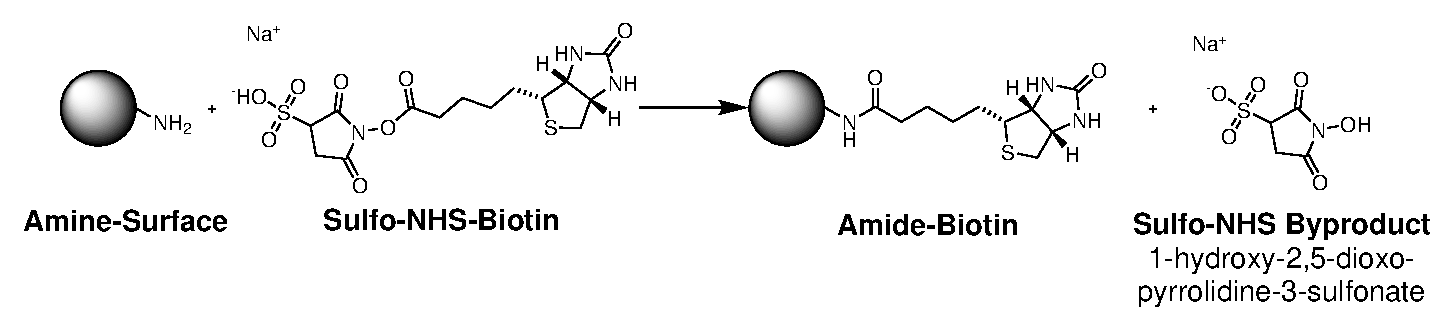
\includegraphics[width=\linewidth]{./Ressources/Chemistry/Sulfo-NHS.eps}
	\capption{Amine Bead Modification with Sulfo-NHS-Biotin}{An amine terminated bead is incubated with sulfo-NHS-Biotin to cover its surface by amide-Biotin. As byproduct the sulfo-NHS-ester 1-hydroxy-2,5-dioxopyrrolidine-3-sulfonate splits off. }
	\label{fig:Chem:NH2-NHS}
\end{figure}


\begin{figure}[htb!]
	\centering
	\subfloat{
		\subfigimg[height=90pt]{a}{./Ressources/Biotinyl/mag-nh2}	
	} \hfill
	\subfloat{
		\subfigimg[height=90pt]{b}{./Ressources/Biotinyl/cooh}	
	}\hfill
	\subfloat{
		\subfigimg[height=90pt]{c}{./Ressources/Biotinyl/IgG-cooh}	
	} \\
\vspace{\baselineskip}
	\subfloat{
	\subfigimg[height=150pt]{c}{./Ressources/Biotinyl/stability}	
	}

	\capption{Titration of Biofunctional Molecules on \SI{8}{\micro\meter} Particles}{ (\textbf{a}) NHS-Biotin, MFI, CV, reduced chi square = 275.19597, Hill Fit $y=Vmax*x^n/(k^n+x^n)$, Vmax = 173.077, k = 0.0572831, n = 1.63554 (\textbf{b}) Amin-PEG$_2$-Biotin MFI, CV, outlier neglected Gleichung: $y=Vmax*x^n/(k^n+x^n)$ Vmax	171,02602, k   	0,04201, n   	0,91338,Chi-Quadr Reduziert	4,07387	(\textbf{c}) MFI, CV, reduced chi square = 0.91011, Hill Fit $y=Vmax*x^n/(k^n+x^n)$, Vmax = 713.83643, k = 182.83011	, n = 0.72458  (\textbf{d}) MFI, SEM, $\tau_{decay}$ = \num{1.42557 +- 0.16188}	Equation	$y = A \exp^\frac{-x}{\tau_{decay}} + y_0$	y0	0.12369 ± 0.01576	A1	0.91263 ± 0.06964	t1	1.42557 ± 0.16188	Reduced Chi-Sqr	0.00542 }
	\label{fig:biotinyl:titration}
\end{figure}



%\begin{figure}[htb!]
%	\centering
%	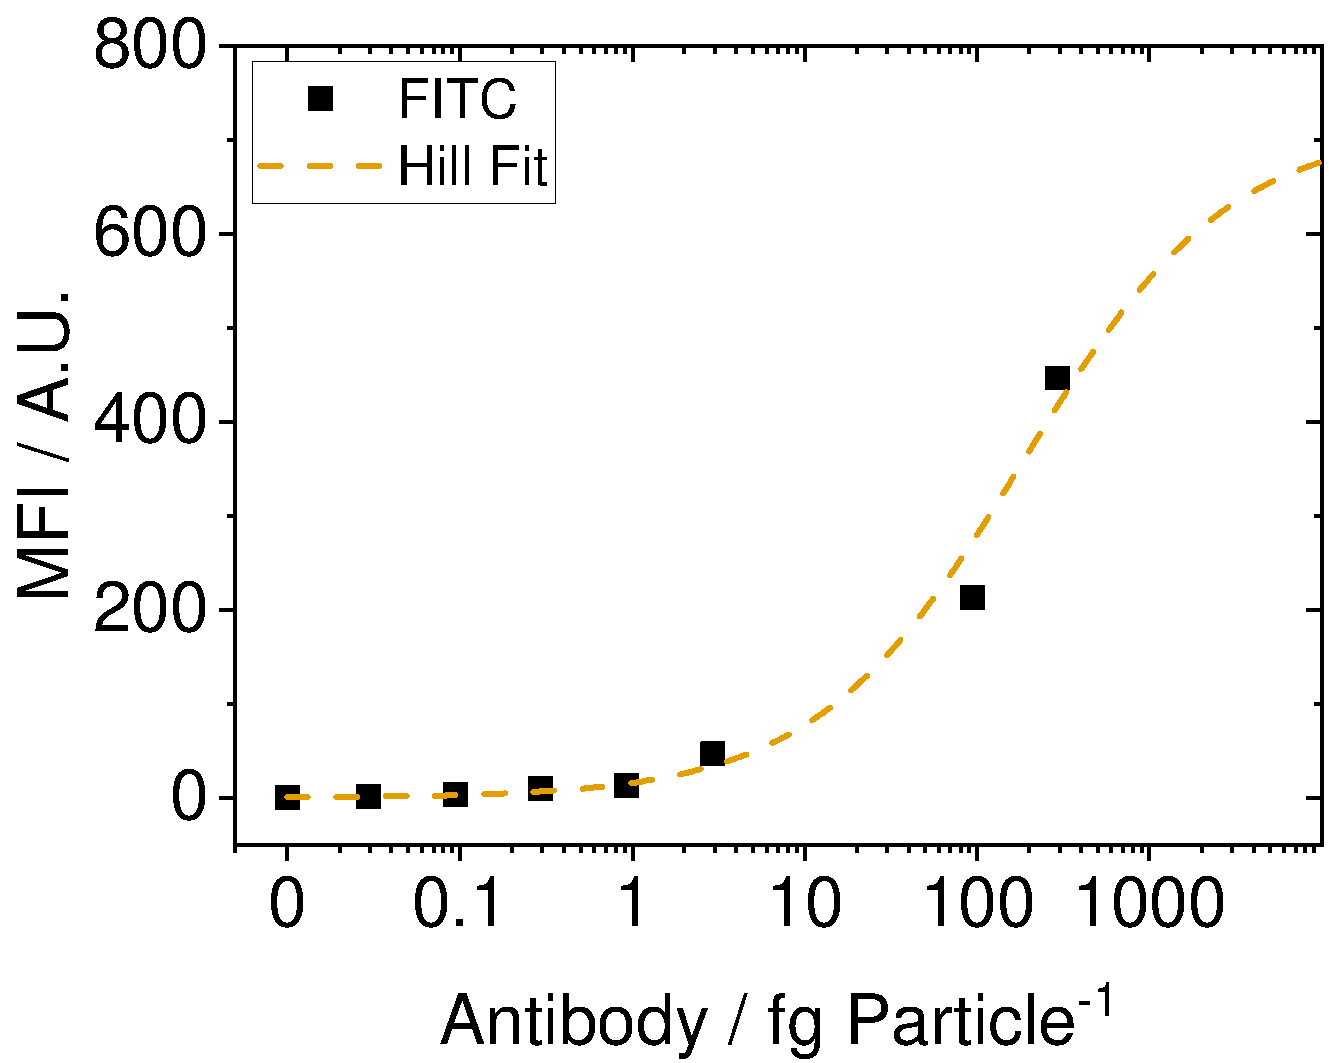
\includegraphics[width=.7\linewidth]{./Ressources/Biotinyl/IgG-cooh}
%	\capption{Titration of Anti-IgG1 on \SI{8}{\micro\meter} Particles}{MFI, CV, reduced chi square = 
%		0.91011, Hill Fit $y=Vmax*x^n/(k^n+x^n)$, Vmax = 713.83643, k = 182.83011	, n = 0.72458 }
%	\label{fig:biotinyl:IgG-cooh}
%\end{figure}

%\begin{figure}[htb!]
%	\centering
%	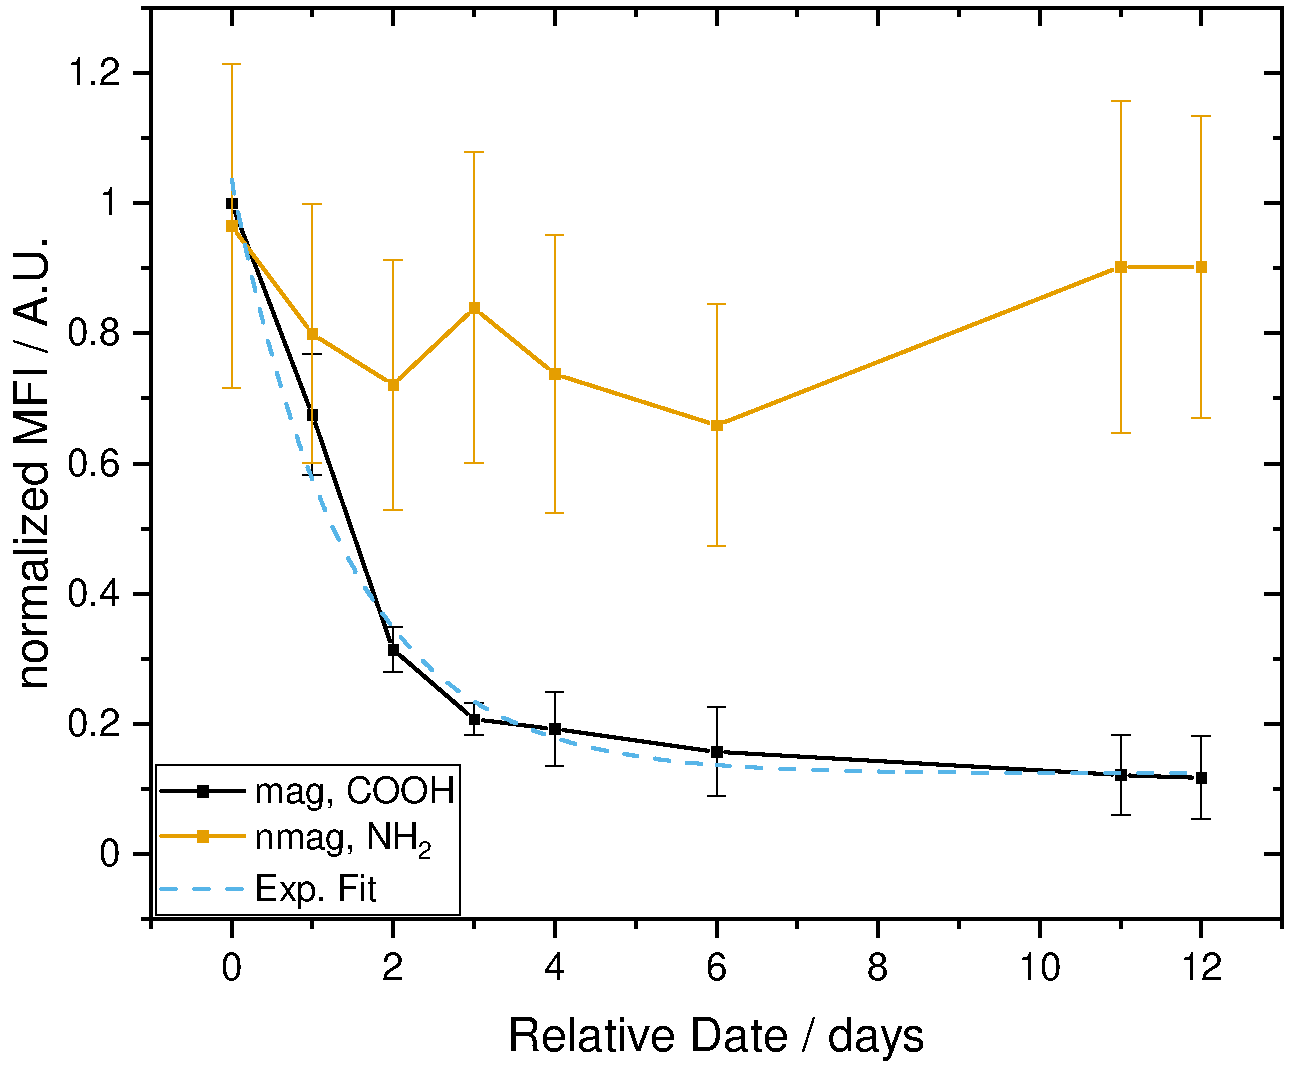
\includegraphics[width=\.7\linewidth]{./Ressources/Biotinyl/stability}
%	\capption{Titration of Anti-IgG1 on \SI{8}{\micro\meter} Particles}{MFI, SEM, reduced chi square = 
%		0.00542, Hill Fit $y=Vmax*x^n/(k^n+x^n)$, Vmax = 713.83643, k = 182.83011	, n = 0.72458 }
%	\label{fig:biotinyl:stability}
%\end{figure}


\section{Concentration Measurements in MRCyte}
Explain v-c
\begin{figure}[htb!]
	\centering
	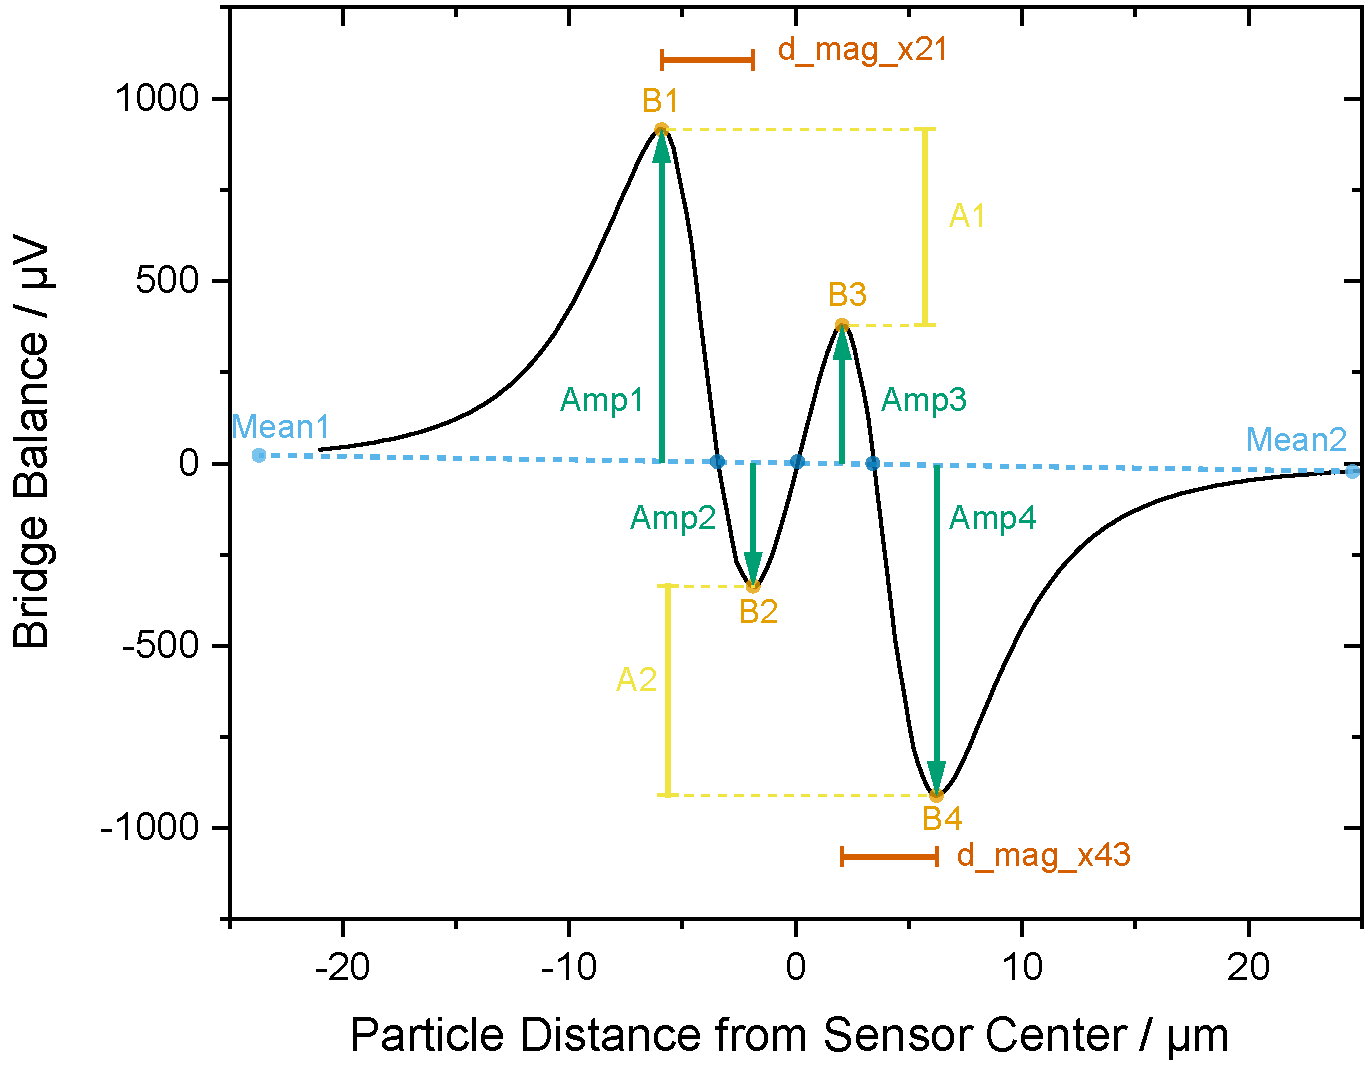
\includegraphics[width=.7\linewidth]{Ressources/Simulation/ExampleSignal}
	\capption{Example Signal of Magnetic Measurement}{explain all}
	\label{fig:conc:example}
\end{figure}

\begin{figure}[htb!]
	\centering
	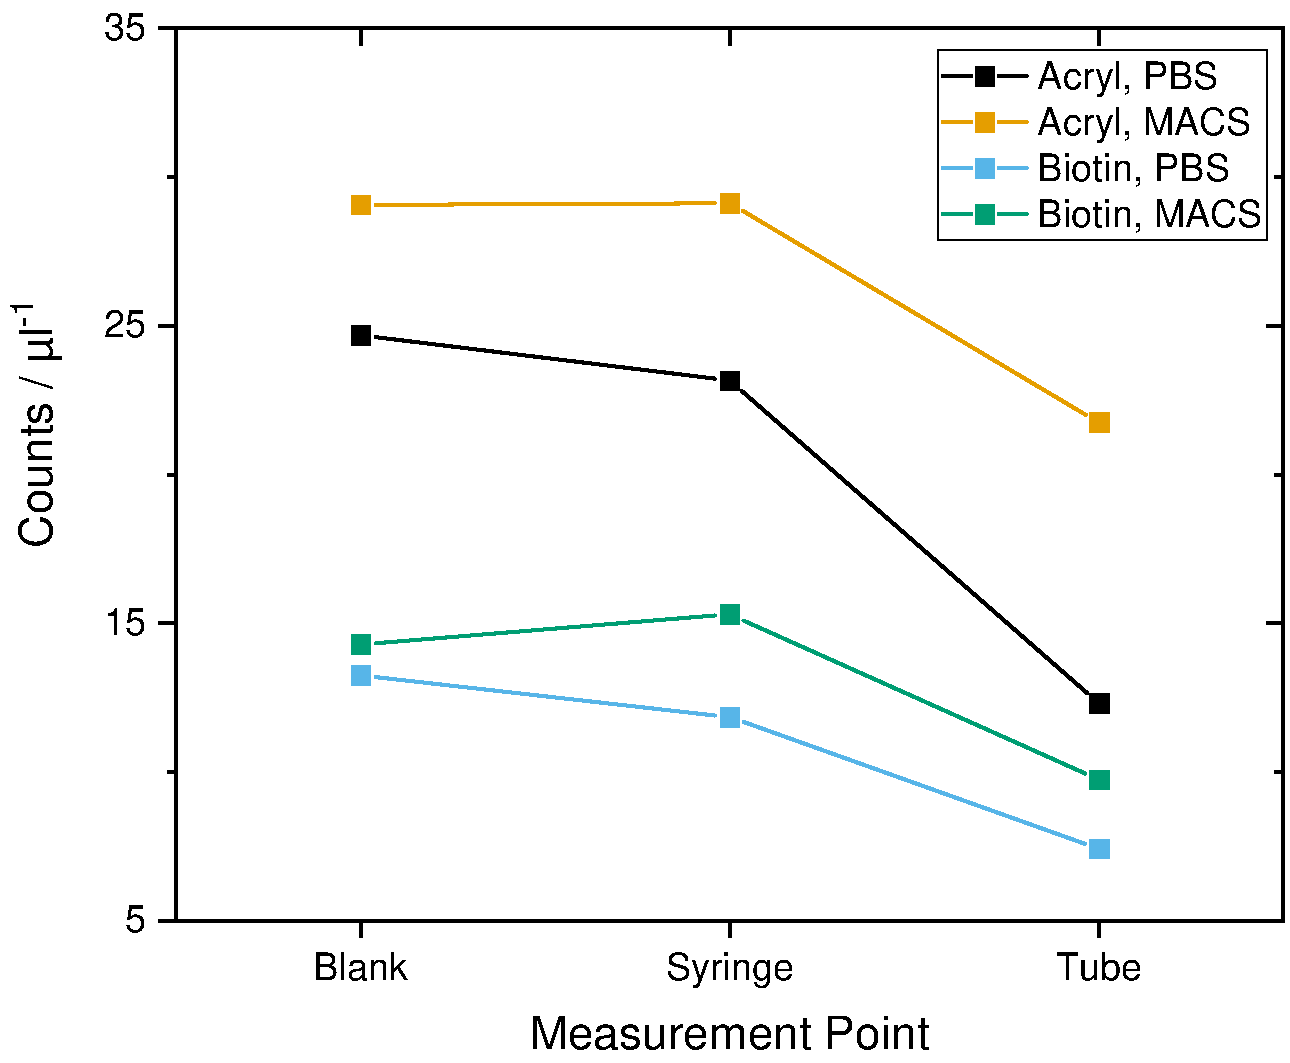
\includegraphics[width=.7\linewidth]{Ressources/Concentration/Losses-Syringe-Tubing}
	\capption{Bead Loss Evaluation in Connectors}{Losses in different buffers and bead surfaces.}
	\label{fig:conc:losses_syringe}
\end{figure}



\subsection{Calibration of Flow Field}
\begin{figure}
	\centering
	\subfloat{
		\subfigimg[height=150pt]{a}{Ressources/Concentration/ConcentrationError}	
	} \hfill
	\subfloat{
		\subfigimg[height=150pt]{b}{Ressources/Concentration/ConcentrationVelocity}	
	}
	\capption{Absolute Concentration Measurements}{Mean from 3 independent measurements(\textbf{a}) mean, sd (\textbf{b}) mean, SEM, Reference Count based error: Liner fit steepness \num{0,34622 +- 0,00968} --> Correction Factor (inverse) \num{2,88833 +- 0,08075}, Velocity Based Correction: $Q/A$ Dims: \SI{700}{\micro\meter}x\SI{50}{\micro\meter} Q = \SI{30}{\micro\liter\per\minute} --> \num{2,26109}}
	\label{fig:conc:AbsConcError}
\end{figure}

\begin{figure}
	\centering
	\subfloat{
		\subfigimg[height=150pt]{a}{Ressources/Concentration/BiotinylWrongCorrection}	
	} \hfill
	\subfloat{
		\subfigimg[height=150pt]{b}{Ressources/Concentration/BiotinylTime}	
	}
	\capption{Error Sources in Concentration Measurements}{(\textbf{a}) mean, SEM Fit factor comparison with protein coated surfaces (\textbf{b}) mean, SEM}
	\label{fig:conc:BiotnylWrongCorr}
\end{figure}

\subsection{Count Stability}
Measurement over 1h

\begin{figure}[!h]
	\centering
	\subfloat{
		\subfigimg[height=150pt]{a}{Ressources/Concentration/BiotinylCountAll}	
	} \hfill
	\subfloat{
		\subfigimg[height=150pt]{b}{Ressources/Concentration/BiotinylTimeAll}	
	}
	\capption{Reproducibility of Concentration Measurements with Saturated Neutravidin Surface}{(\textbf{a}) \SI{80}{\micro\liter\per\minute} mean, SEM (\textbf{b}) All,mean, SEM,}
	\label{fig:conc:All}
\end{figure}



\begin{figure}[htb!]
	\centering
	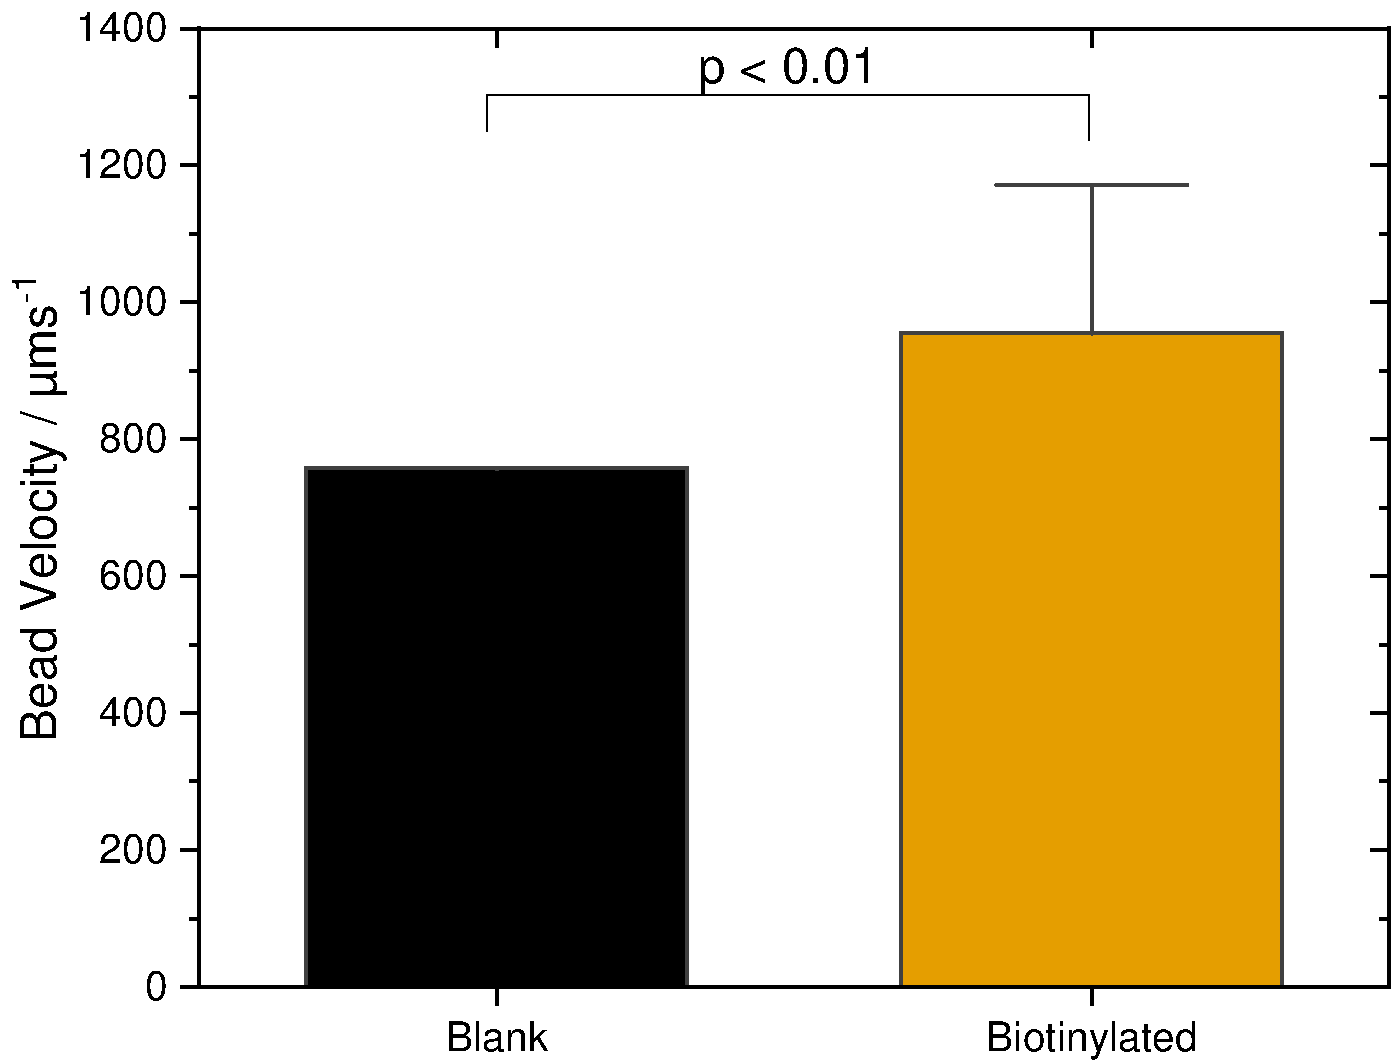
\includegraphics[width=.7\linewidth]{Ressources/Concentration/CaptureVelocity}
	\capption{Measured Bead Velocity}{ p < 0.01}
	\label{fig:conc:vel}
\end{figure}




\subsubsection{Concentration Measurement in Diluted Whole Blood}


\begin{figure}[htb!]
	\centering
	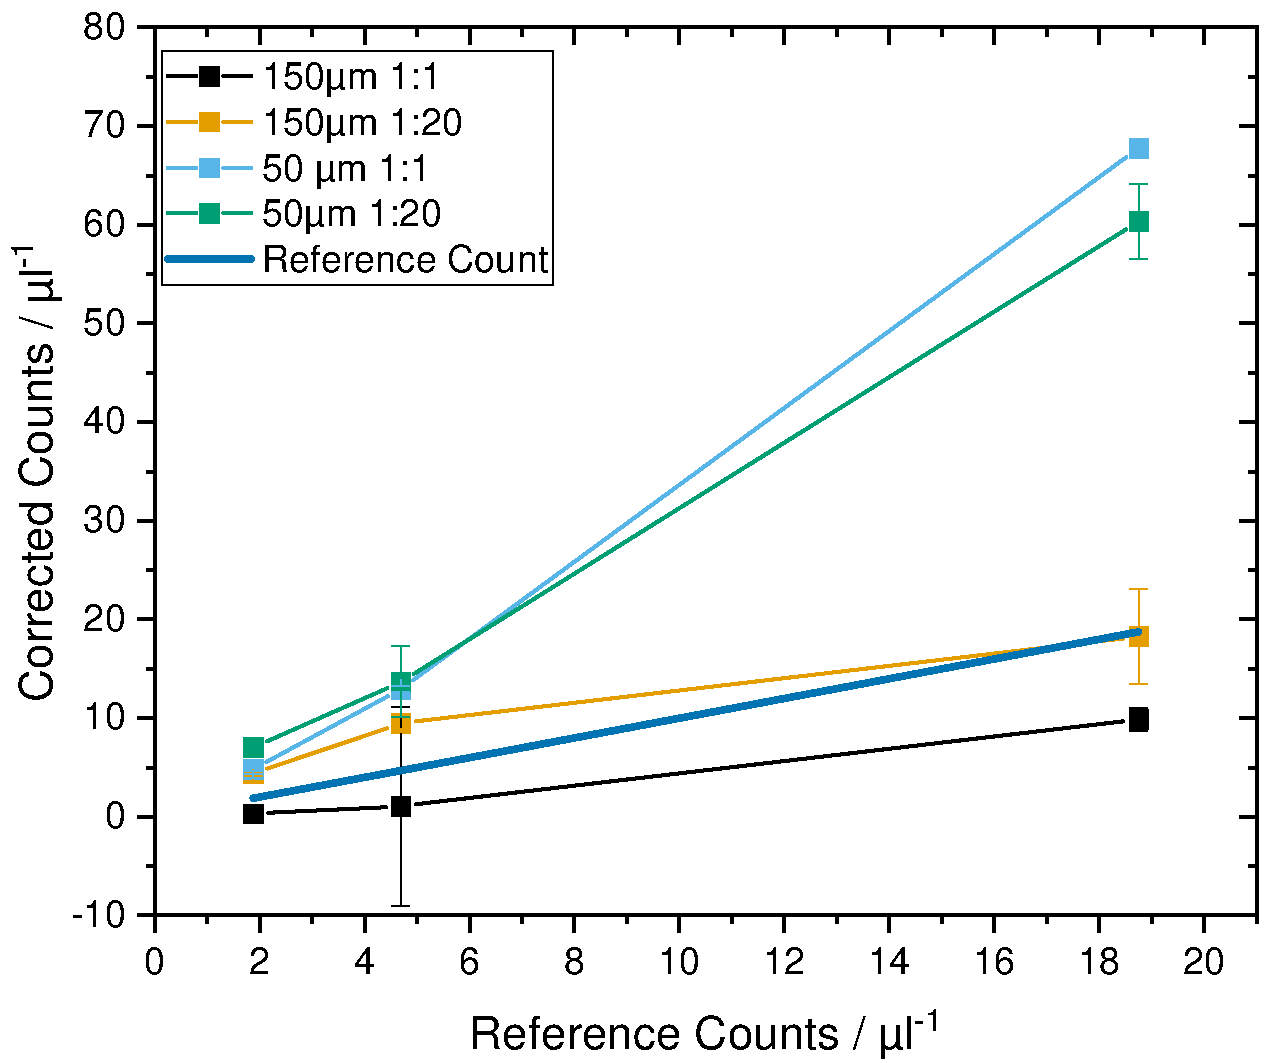
\includegraphics[width=.7\linewidth]{Ressources/Concentration/CorrectionBlood}
	\capption{Absolute Concentration Measurement in Blood Samples Under Varying Channel Height}{Velocity Correction does not work for high concentrations in \SI{50}{\micro\meter}}
	\label{fig:conc:blood}
\end{figure}




\subsection{Differential Counting Setup}

\subsubsection{Sensitivity Calibration}

\begin{figure}[!h]
	\centering
	\subfloat{
		\subfigimg[height=150pt]{a}{Ressources/Differential/Optupper}	
	} \hfill
	\subfloat{
		\subfigimg[height=150pt]{b}{Ressources/Differential/Optlower}	
	}
	\capption{Hysteresis Calibration for Stacked \Gls{pcb} }{(\textbf{a}) Optimized for top sensor (\textbf{b}) Optimized for bottom sensor}
	\label{fig:diff:sensitivity}
\end{figure}

\subsubsection{Concentration Measurement in Buffer Solution}



\begin{figure}[!h]
	\centering
	\subfloat{
		\subfigimg[height=150pt]{a}{Ressources/Differential/Bottom}	
	} \hfill
	\subfloat{
		\subfigimg[height=150pt]{b}{Ressources/Differential/Top}	
	}
	\capption{Flow Rate Dependency of Counting Setup}{(\textbf{a}) Optimized for top sensor (\textbf{b}) Optimized for bottom sensor}
	\label{fig:diff:flowRate}
\end{figure}

\begin{figure}[htb!]
	\centering
	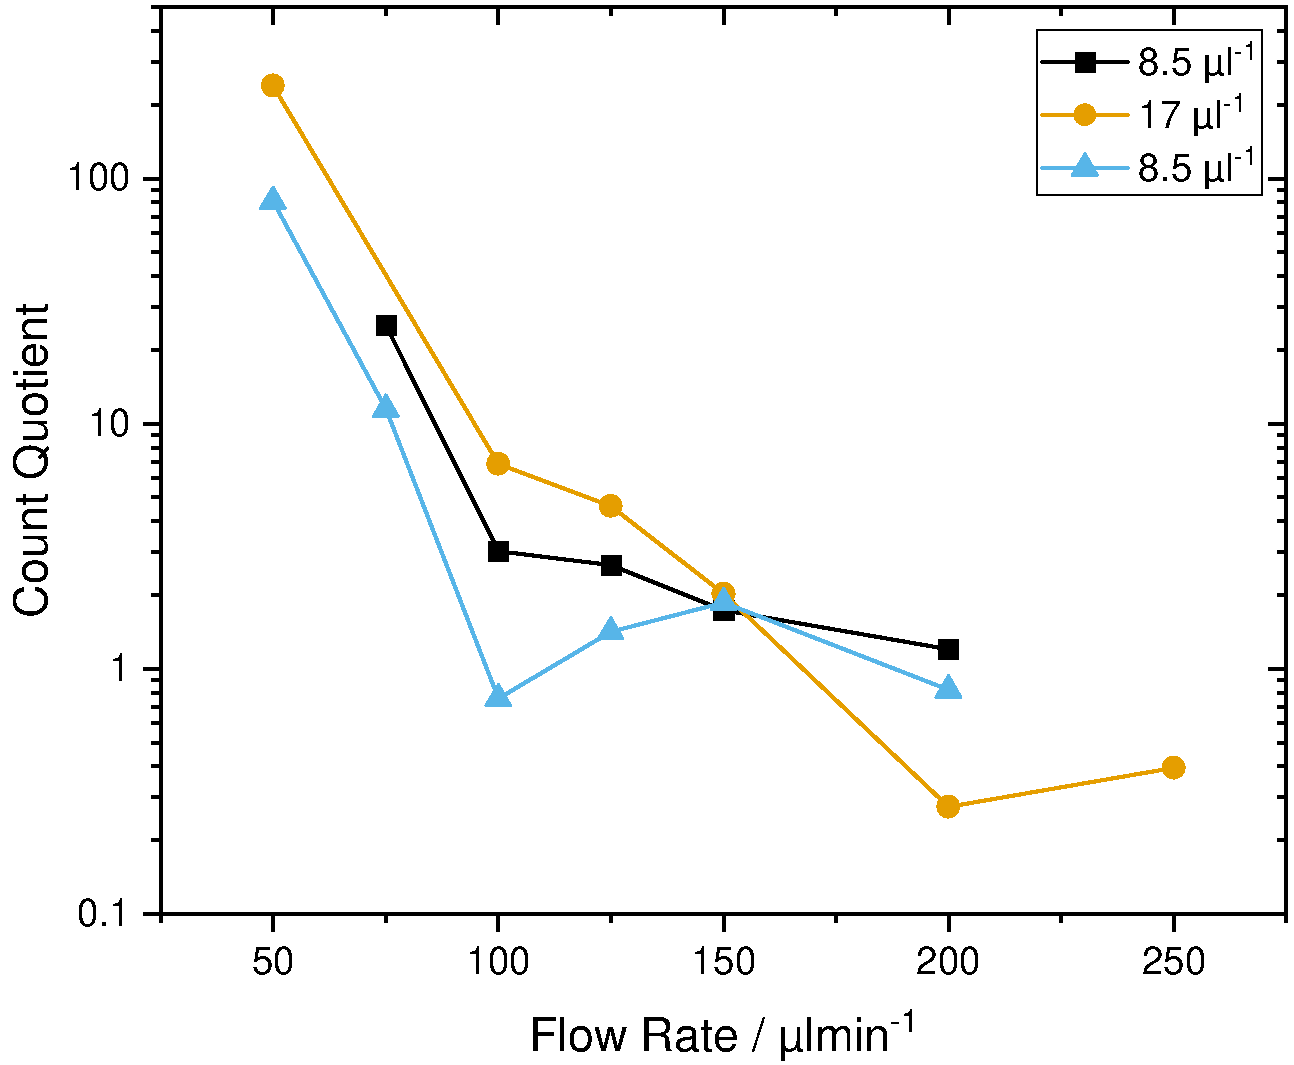
\includegraphics[width=.7\linewidth]{Ressources/Differential/Differential}
	\capption{Optimal Differential Counting Flow Rate}{Losses in different buffers and bead surfaces.}
	\label{fig:conc:optimum}
\end{figure}




\subsection{Surface Magnetization of Biofunctionalized Beads}

Somehow BNF-Dextran showed unspeficity initally, but not anymore later on

\begin{figure}[!h]
	\centering
	\subfloat{
		\subfigimg[height=150pt]{a}{Ressources/Concentration/BNFC1}	
	} \hfill
	\subfloat{
		\subfigimg[height=150pt]{b}{Ressources/Concentration/BNFVc}	
	}
	\capption{Bead Coverage Assay with BNF-Dextran-redF-\SI{100}{\nano\meter}}{(\textbf{a}) 1. \SI{80}{\micro\liter\per\minute} 2. \SI{40}{\micro\liter\per\minute} 3. \SI{20}{\micro\liter\per\minute} 4. \SI{10}{\micro\liter\per\minute} (\textbf{b}) d = \SI{8}{\micro\meter}}
	\label{fig:conc:BNF}
\end{figure}



\begin{figure}[!h]
\centering
\subfloat{
	\subfigimg[height=150pt]{a}{Ressources/Concentration/OceanC1}	
} \hfill
\subfloat{
	\subfigimg[height=150pt]{b}{Ressources/Concentration/OceanVc}	
}
\capption{Bead Coverage Assay with OceanNanotec \SI{50}{\nano\meter}}{Mean from 3 different particle distributions at maximum coverage, SEM(\textbf{a}) d = \SI{4}{\micro\meter} (\textbf{b}) d = \SI{8}{\micro\meter}}
\label{fig:conc:Ocean}
\end{figure}


\section{Surface Modification and Biofunctionalization of the Sensor Chip Substrate}

\subsection{Physisorption}
Quantification in Plate Reader
Trial with Neutravidin + Sensor (Esthis Versuch)
\clearpage

\begin{figure}
	\centering
	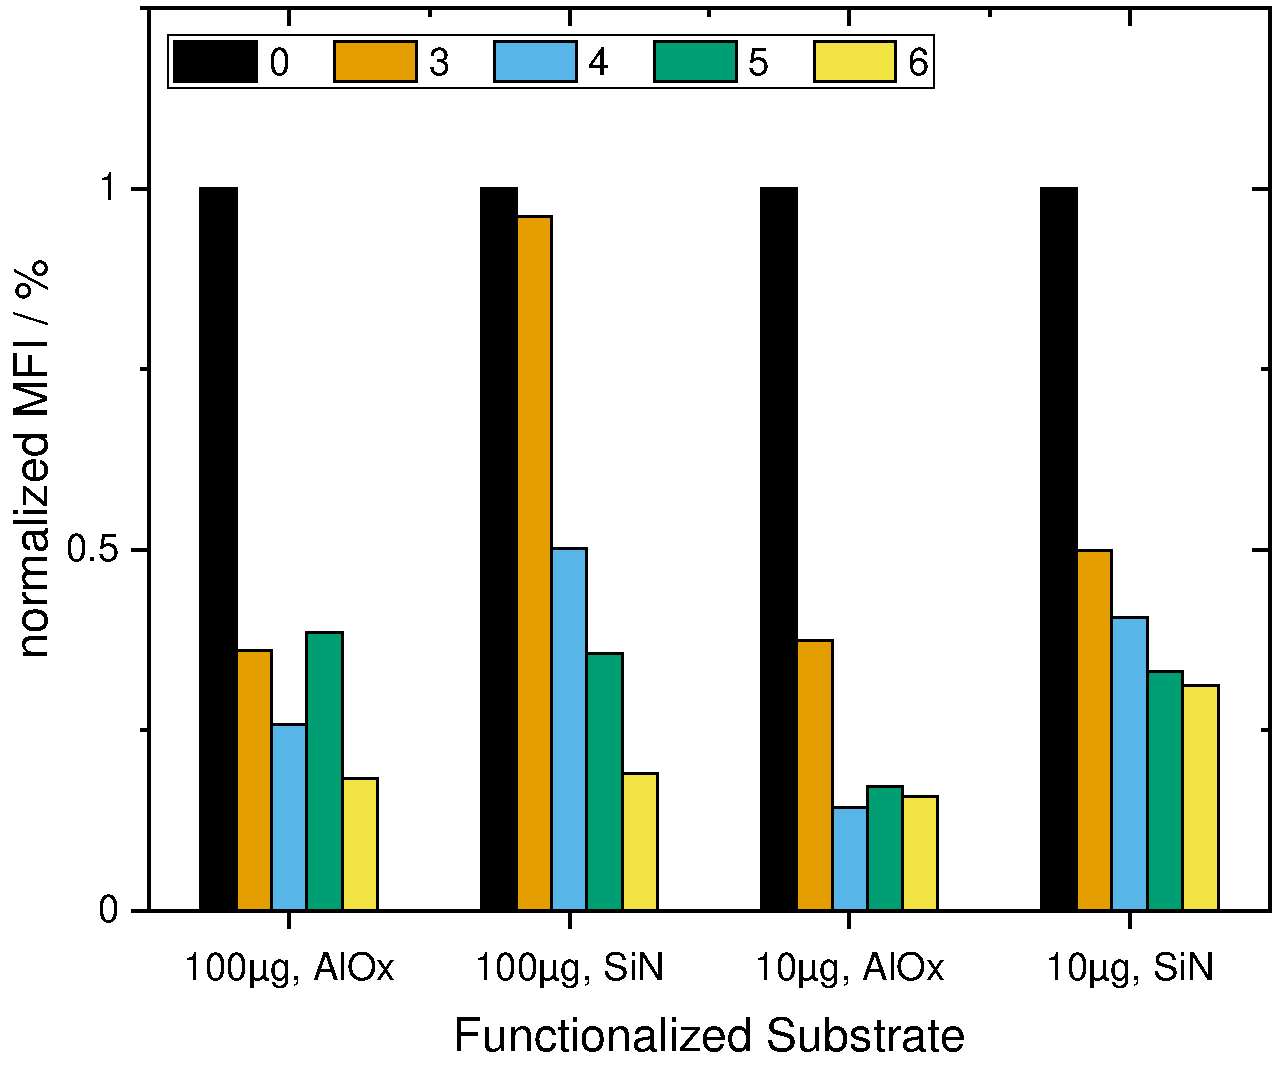
\includegraphics[height=150pt]{Ressources/ResultPlots/SurfaceFuncSiNAlOx}
	\capption{Surface Adsorption Stability of Neutravidin on \Gls{sin} and \Gls{alox}}{Blank with PBS and Blank substrate, corrected, then normalized, absolute protein per \textasciitilde \SI{25}{\milli\meter\square}}
\end{figure}


\subsection{Covalent Attachment}
\clearpage


\begin{figure}[htb!]
	\centering
	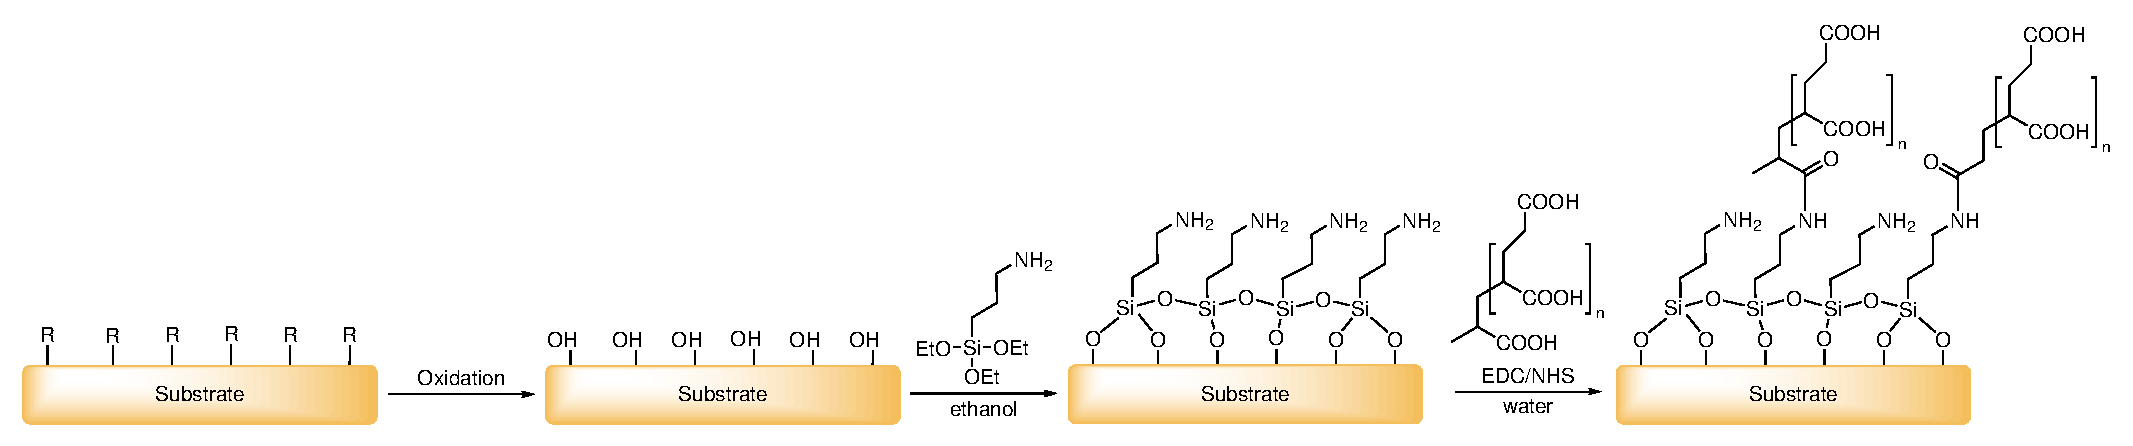
\includegraphics[width=1\linewidth]{Ressources/Chemistry/Substrate}
	\capption{General process chain of chemical surface modification}{Any substrate with various surface groups R (\textbf{a}) is oxidized to exhibit \gls{hydroxyl} groups.(\textbf{b}). Then a silane \gls{sam} is attached (\textbf{c}) and subsequently modified by carbodiimide chemistry with \gls{paa}. (\textbf{d})}
	\label{fig:chem:func:withPAA}
\end{figure}
\subsubsection{Plasma-Based Approach}

\begin{figure}
	\centering
	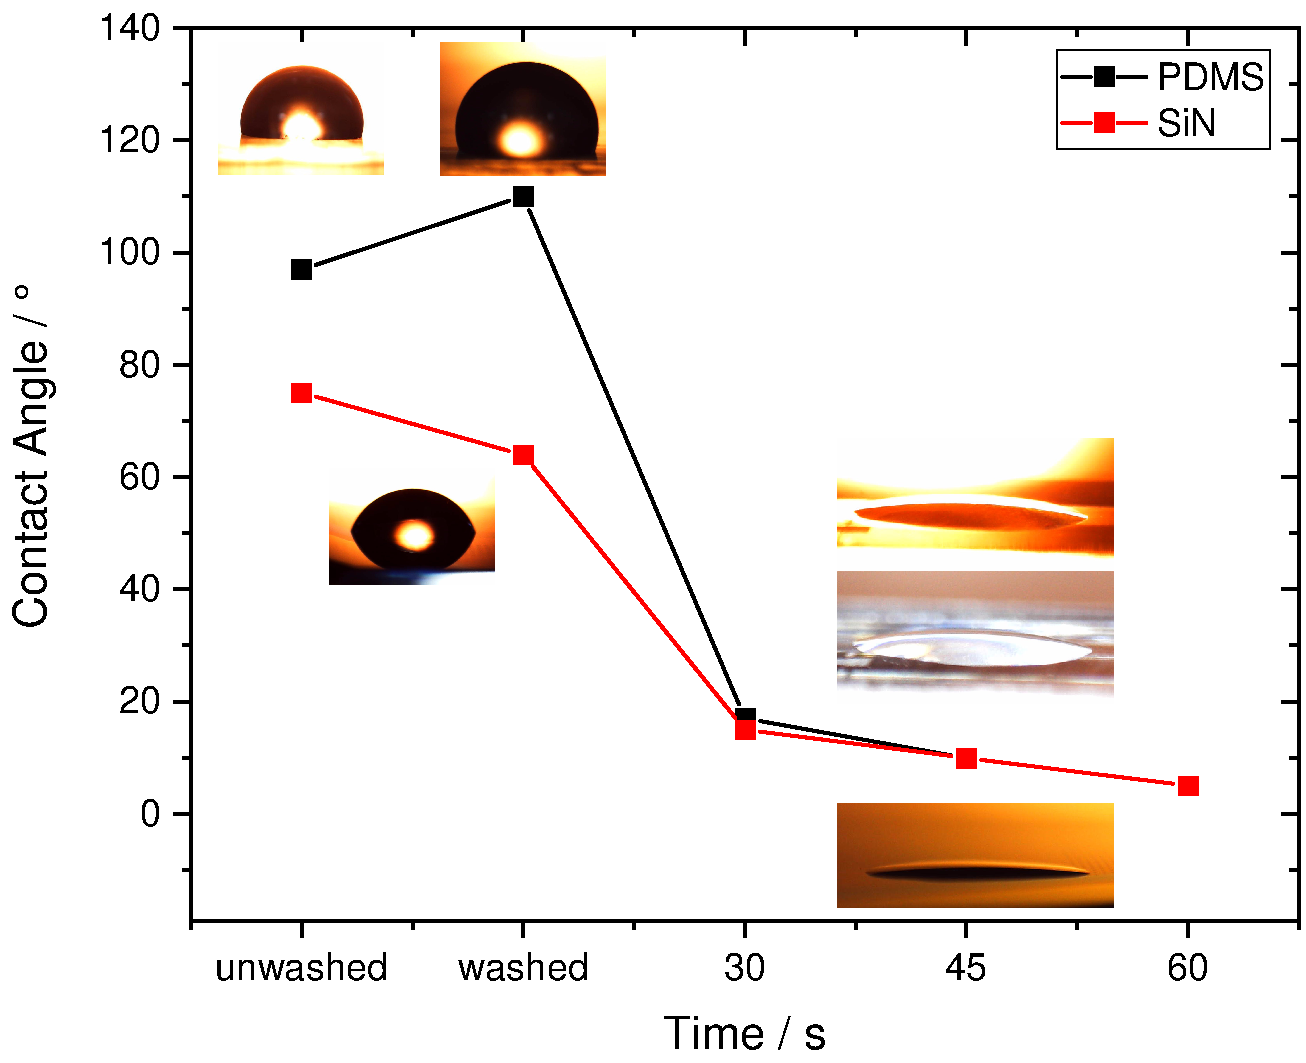
\includegraphics[height=150pt]{Ressources/ResultPlots/PDMS-sessileDrop}
	\capption{Hydrophbicity Analysis of \gls{pdms} under Plasma Exposure}{test123}
\end{figure}

\subsubsection{Water-Based Approach}
Sonicate in Acetone and Water 5'
1:1 \gls{hcl}:Methanol
\gls{h2so4}
Treat for 30 min in light boiling water